% =========================================================
% Rational Approximation on the Number Line
% =========================================================

\begin{figure}[h]
\centering
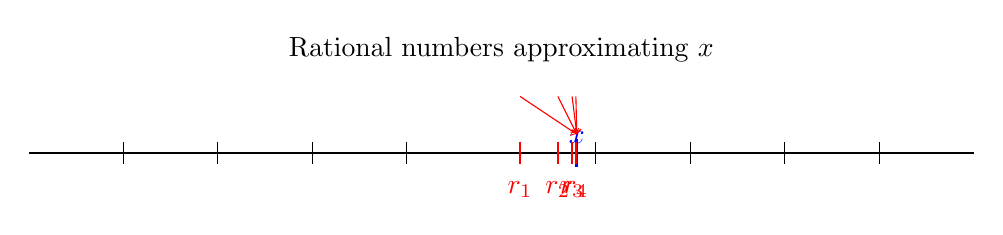
\begin{tikzpicture}[scale=1.2]

% Number line
\draw[thick] (-5,0) -- (5,0);

% Tick marks
\foreach \x in {-4,-3,-2,-1,1,2,3,4}
{
  \draw (\x,0.12) -- (\x,-0.12);
}

% Real number x
\draw[very thick,blue] (0.8,0.15) -- (0.8,-0.15);
\node[above,blue] at (0.8,0) {$x$};

% Rational approximations
\draw[thick,red] (0.2,0.12) -- (0.2,-0.12);
\node[below,red] at (0.2,-0.2) {$r_1$};

\draw[thick,red] (0.6,0.12) -- (0.6,-0.12);
\node[below,red] at (0.6,-0.2) {$r_2$};

\draw[thick,red] (0.75,0.12) -- (0.75,-0.12);
\node[below,red] at (0.75,-0.2) {$r_3$};

\draw[thick,red] (0.79,0.12) -- (0.79,-0.12);
\node[below,red] at (0.79,-0.2) {$r_4$};

% arrows showing convergence
\draw[->,red] (0.2,0.6) -- (0.8,0.2);
\draw[->,red] (0.6,0.6) -- (0.8,0.2);
\draw[->,red] (0.75,0.6) -- (0.8,0.2);
\draw[->,red] (0.79,0.6) -- (0.8,0.2);

\node at (0,1.1) {Rational numbers approximating $x$};

\end{tikzpicture}

\caption{Rational numbers approximating a real number $x$. The rational values
$r_1,r_2,r_3,r_4,\dots$ approach $x$ with decreasing error.}
\label{fig:rational-approximation}
\end{figure}




\begin{remark}[Geometric view of rational approximation]

Let $x$ be a real number.  The density of the rational numbers implies
that we can find rational numbers arbitrarily close to $x$.

Thus we may construct a sequence

\[
r_1,r_2,r_3,\dots
\]

of rational numbers satisfying

\[
|x-r_n| \to 0.
\]

Geometrically this means that the rational numbers $r_n$ approach the
point $x$ on the number line.  Even if $x$ is irrational, rational
numbers can approximate it arbitrarily closely.

\end{remark}


\begin{remark}[Approximating $\sqrt{2}$]

There exist rational numbers whose squares are less than $2$ and others
whose squares are greater than $2$.

These two families of rational numbers approach $\sqrt{2}$ from below
and above:

\[
1.4 < 1.41 < 1.414 < \sqrt{2} < 1.415 < 1.42 < 1.5.
\]

Although these rational numbers become arbitrarily close to $\sqrt{2}$,
none of them equals $\sqrt{2}$.

Thus the rational number system contains a gap at $\sqrt{2}$.

\end{remark}
